\cleardoublepage
\setcounter{chapter}{2} %The counter for chapters should be set one less than 
                        %the actual chapter number, for example, {1} for 
                        %chapter 2, and {2} for chapter 3.
\setcounter{section}{3} %The counter for sections should be set to match the
                        %actual chapter number, for example, {2} for sections 
                        %in chapter, and {3} for sections in chapter 3. 
\chapter{GUI Command Buttons and Parameters}
\markboth{WEBGUI USERS' GUIDE}{GUI COMMAND BUTTONS AND PARAMETERS}
\pagenumbering{arabic}
\setcounter{page}{33} %The counter for page numbers must be placed here in your
                     %chapter, following the \chapter and \markboth commands.
                     %It should always be the next available right-hand page.
                     %All chapters start on new rights. It will always be
                     %an odd number.  

 
\section{Introduction}
\label{sec:3-2}
The purpose of a graphical interface is to control some software and display output. Presumably the software 
has a variety of routines (tasks it can perform). And with each routine, there can be associated parameters 
(variables). Therefore, it would be helpful if the GUI can view and change parameters before requesting that a 
routine to be executed. After execution, the GUI should be able to display text and graphical output.

If you only use the command line version of \f{WEBGUI}, you do not need to read this section. If however, you
would like to call \textbf{webinit} to add command buttons and parameter storage in your web browser, then
this section explains how that works.

In order for the web browser interface to provide command buttons and store parameters for viewing and changing,
you must inform the web browser about your software's routines and variables. You accomplish this with the 
\textbf{webinit} call which is described in Section \ref{sec:2-1}.

\section{Calling webinit}
\label{sec:3-1}
The argument of \textbf{webinit} is an array of strings (each 80 characters in length). 
This section describes the formatting of these strings.
There are 4 types of argument strings. Strings that begin with the letter "c" define command buttons. Strings
that begin with the letter "n" define a parameter. Strings that begin with the letter "r" define an association
between a command and a parameter. And strings that begin with the letter "s" define a list of options for
a parameter. All strings have the same format. Each begins with a single letter (either c, n, r, or s) and then each
has a list of key = value pairs separated by commas. Spaces are optional.

Below is the example array of strings we presented in Section \ref{sec:2-1}. These strings create 3 command buttons, 
store 4 parameters (2 integers, 1 real, and 1 string) and provide 3 options for 1 of the parameters. Notice the 4 types 
of strings and the common format. We will explain this example in the 4 sections to follow:
\begin{verbatim}
    char str[14][80] = {
        "c c=BuildTire, k=t",
        "c c=BuildEngine, k=e",
        "c c=AssembleCar, k=c",
        "n n=TireRadius, a=tr, t=r, i=1, d=12.5",
        "n n=TireColor, a=tc, t=s, i=1, d=red",
        "n n=EngineSize, a=es, t=i, i=1, d=300",
        "n n=CarColor, a=cc, t=i, i=2, d=1",
        "r c=BuildTire, n=TireRadius",
        "r c=BuildTire, n=TireColor",
        "r c=BuildEngine, n=EngineSize",
        "r c=AssembleCar, n=CarColor",
        "s n=CarColor, v=0, l=red",
        "s n=CarColor, v=1, l=white",
        "s n=CarColor, v=2, l=blue"
    };
 \end{verbatim}

\subsection{Command buttons}
\label{sec:3-3}
%\begin{table}[htbp]
\begin{center}
\begin{tabular}{|l|l|l|l|}
\hline
\multicolumn{3}{|c|}{\strutul Key-value pairs associated with $c$ string} \\
\hline 
\strutul
Name & Key & Value \\
\hline
\strutu
command button text & c & maximum of 20 characters \\
abbreviation & k & maximum of 3 lowercase characters \\
\hline
\end{tabular}
\end{center}
%\caption{Syntax for $c$ string.}
%\label{table-1}
%\end{table}

Every string that begins with "c" will create a command button in the web browser GUI. The name on the button is the value 
associated with the key c. When this button is pushed, a command string is generated and placed
in the command string buffer. (Your software retrieves this command string when it calls \textbf{webreadline}.)

The format of the generated command string is as follows. The first 1-3 characters will be the abbreviation that you assigned
to that command via the key-value pair of k. The remainder of the command string will be key-value pairs separated by 
commas. The keys will be parameter names that you define with an $n$ string (and associate with an $r$ string) and the 
values will be any parameters that you changed from their defaults with the web browser drop down menus.

For example, if you push the button "Build Tire", the command string transmitted will be an 80 character string with the first letter "e"
and the remaining 79 characters as spaces. If before you push the button "Build Tire", you change the associated parameter
"TireRadius" from its default of 12.5 to 13.5, and "TireColor" from red to while, then the transmitted command string will be 
\begin{verbatim}
e TireRadius=13.5, TireColor=white 
\end{verbatim}
padded out with spaces to length 80.

\subsection{Parameters}
\label{sec:3-4}

\begin{center}
\begin{tabular}{|l|l|l|l|}
\hline
\multicolumn{3}{|c|}{\strutul Key-value pairs associated with $n$ string} \\
\hline 
\strutul
Name & Key & Value \\
\hline
\strutu
parameter name & n & maximum of 20 characters \\
abbreviation & a & maximum of 3 characters \\
data type & t & i (int), r (real), s (string), f (file)\\
\strutl
index & i & pointer to \f{IP}, \f{RP}, \f{SP} \\
default value & d & maximum of 40 characters/digits \\
\hline
\end{tabular}
\end{center}

Every string that begins with "n" will define a parameter for the web browser to store and allow the user to view and change.
When a user changes a parameter via a web browser drop down menu, the new value of that parameter is transmitted
when the associated command button is pressed. (This is described in the subsection prior and following.)

Changed parameter values are also transmitted when you close the drop down menu but have not actually issued the 
associated command. If you close a drop down menu where a parameter has been changed, then a command string
is placed in the command string buffer. This isn't a normal command string. The first 1-3 characters of the command string
are the capital letter version of the associated command abbreviation. It is important that your software is aware of this
and processes these slightly different command strings correctly after receiving them from \textbf{webreadline}. For
example, if you change the parameter "TireRadius" from its default of 12.5 to 13.5, and "TireColor" from red to while, and
then you close the drop down menu (without issuing the "BuildTire" command), then the following command string will be
transmitted:
\begin{verbatim}
E TireRadius=13.5, TireColor=white 
\end{verbatim}
Note that this differs from the command string in the preceding subsection which started with a lowercase "e".

The web browser recognizes 3 types of parameters; integer, real, and string. Strings come in 3 types,  (i) contain
no space characters, (ii) contain space characters, and (iii) file names. If you declare a string as a file name, then the web browser 
will give you a file selection dialog box to change them. Declare a parameter's type by using the key-value pair associated with
t. For a number, set the value to either i or r denoting integer or real respectively. For a string, set the value to either s, l, or f
to denote the string has no spaces, the string has spaces, and file name.  

The web browser also assumes that your software maintains these variables (integers, reals, strings) in 3 arrays, \f{IP}, \f{RP},
\f{SP}. Therefore each parameter that you let the web browser know about needs an index into your software's associated 
\f{IP}, \f{RP}, \f{SP} array. The first integer variable in your software's \f{IP} array is referred to as 1, not 0. The second is 2, not 1, etc. 
When you declare a parameter with an $n$ string, the key-value pair associated with $i$ should be the index of that
parameter in your software's associated array. Indices for integers, reals, and strings are independent
of each other and all start at 1. It is significant to match these correctly so that future calls to 
\textbf{webupdate(ip,rp,sp)} can update (change) the correct parameters in the web browser.

For each parameter that you associate with a command (explained in the next subsection), you should provide a default
value with the key-value pair associated with d. If you wish to provide a default string that contains spaces, then surround
the default string with quotation marks, otherwise quotation marks are optional.

\subsection{Associate parameters with commands}

\begin{center}
\begin{tabular}{|l|l|l|l|}
\hline
\multicolumn{3}{|c|}{\strutul Key-value pairs associated with $r$ string} \\
\hline 
\strutul
Name & Key & Value \\
\hline
\strutu
command name & c & maximum of 20 characters \\
parameter name & n & maximum of 20 characters \\
\hline
\end{tabular}
\end{center}

Any parameter that you would like a user to be able to view and change must be associated with a command. You
associate a parameter with a command with a string that begins with "r". Each command button has a smaller button
beside it with a plus-sign on it. Pressing this button opens a drop down menu revealing all the parameters associated
with a command. You may associate a parameter with more than 1 command. Figure \ref{fig:3} shows the result of our
example here after the user opened a drop down menu. 
Command "BuildTire" has 2 parameters associated with it. Pressing the plus-sign button beside the
"BuildTire" button opens a drop down menu containing the parameters "TireRadius" and "TireColor". Figure \ref{fig:12}
also shows the result of our example here. In this Figure, the user opened the "AssembleCar" drop down menu and
then opened the "CarColor" options menu.

\subsection{Options for parameters}

\begin{center}
\begin{tabular}{|l|l|l|l|}
\hline
\multicolumn{3}{|c|}{\strutul Key-value pairs associated with $s$ string} \\
\hline 
\strutul
Name & Key & Value \\
\hline
\strutu
parameter name & n & maximum of 20 characters \\
hidden value & v & maximum of 40 characters/digits \\
display name & l & maximum of 40 characters/digits \\
\hline
\end{tabular}
\end{center}

If you would like the user to see possible options for a given parameter, then for each such option, provide a string that
starts with the letter "s". Below is our example where we provide the 3 options of red, white, blue for parameter
CarColor. The hidden values are 0, 1, 2 respectively. That means that if a user selects the color blue, then the parameter
CarColor will be set to the integer 2. The user gets a drop down menu when they click on the name of the parameter.
See Figure \ref{fig:12}.
\begin{figure}[H]
\centering
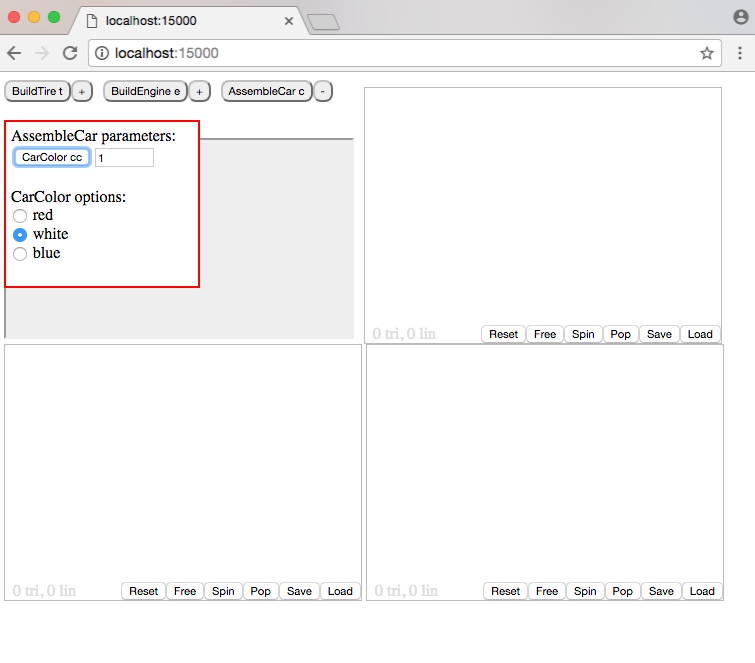
\includegraphics[width=0.75\textwidth]{pix/buttons3.png}
\caption{\f{WEBGUI} after calling \textbf{webinit} to create 3 command buttons, and 1 parameter with 3 options.}
\label{fig:12}
\end{figure} 
